\documentclass{article}

\usepackage{graphicx} % Required for inserting images
\usepackage[a4paper, total={6in, 8in}]{geometry}
\usepackage{parskip} % Required to stop indenting new paragraphs
\usepackage{amssymb}
\usepackage{amsmath}
\usepackage{algpseudocode}
\usepackage{algorithm}
\usepackage[numbers]{natbib} % number references and natbib for more styles
\bibliographystyle{unsrtnat} % sets bibliography to vancouver style

\title{Reverse Mode Algorithmic Differentiation}
\author{cf1021, sam221, aml21, mf621}
\date{}

\begin{document}

\maketitle
\tableofcontents
\newpage
\section{Introduction}

Possibly the broadest issue we have with applying mathematical theory on a computer is that computers can only work with discrete values and since the very essence of a derivative includes $\lim_{x \to 0}$ we immediately run into issues. Immediately when trying to solve this problem one considers first principles where we set a small value $\epsilon$ and then compute the equation:

\begin{equation*}
    \frac{f(x+\epsilon) - f(x)}{\epsilon}
\end{equation*}

This method is called the Finite Differences method. This can give us good approximations however has some drawbacks, the first of all being we have to set $\epsilon$, and an optimal value for this may change depending on our function and our value $x$ and another being that we will never be exact and always have an error, sometimes many orders higher than machine epsilon. Another common method that is used is symbolic differentiation, which takes mathematical expressions and finds their derivatives from a set of rules much like you or I would do on paper. This method although very accurate is tricky to implement, especially with larger functions, and will slow on multivariate functions when trying to compute all the partial derivatives.

In this paper, we will be discussing algorithmic or automatic differentiation, this method breaks down a function into all its elementary operations and applies the chain rule to compute the derivative. Specifically, we will be looking at the reverse mode of algorithmic differentiation as it computes the derivates an order n faster than the forward mode, with n being the number of inputs to the function.

The use of derivatives in algorithms is increasingly clear as artificial intelligence develops and proves its own uses. This is because of backpropagation which is a method used to train neural nets. On these neural nets, one has many nodes connected by a series of weights, such that the change in one value affects the change in another, to optimise these weights we must use a method called gradient descent which requires us to find a derivative.

When solving non-linear systems one method is Newton-Raphson in which iterates are calculated, given an initial $x_0$, using
\begin{equation}
\mathbf{x_{n+1}} = \mathbf{x_n} - [f'(\mathbf{x_n})]^{-1}f(\mathbf{x_n})
\end{equation}
where
\begin{equation}
    f'(\mathbf{x}) = \begin{bmatrix}
        \frac{\partial f_i}{\partial }
    \end{bmatrix}
\end{equation}
 
Hence the computation of derivatives of functions is key to finding the solutions of non-linear systems.

Computing algorithms like Newton-Raphson effectively is necessary to later carry out weight optimization when working with neural nets. We see this when minimizing things like the sum of residual squares, we must first compute a derivative with respect to our weight if we want to find the minimum.

\section{Basics of Computing Derivatives}

There are three common ways to differentiate a function on a computer: numerically, symbolically, and algorithmically. The latter which we will be discussing in depth in this paper. Notably focusing on reverse mode algorithmic differentiation (AD). In contrast to symbolic and algorithmic differentiation, numerical differentiation results in an approximation for the derivative.

The most common example of numerical differentiation is the finite differences method. For \\ $f: \mathbb{R}^n \longrightarrow \mathbb{R}^m$ a partial derivative can be approximated using a truncated Taylor series around $p \in \mathbb{R}^n$. From \cite{chem}
\begin{equation*}
    \frac{\partial f_i (p)}{\partial x_j} \approx \frac{f_i(p+he_j) - f_i(p)}{h}
\end{equation*}
This calculation for the derivative is approximate due to the error in the truncated Taylor series. The run time complexity of using finite differences to calculate all the partial derivatives of $f_i$ with respect to all $x_j$ is $\mathcal{O}(n)$ \cite{dhamarticle}. thus, finite differences is unsuited for systems with a large number of unknowns.

Symbolic differentiation involves taking an algebraic expression and computing its derivative with respect to a specified variable through repeated application of basic rules of calculus using computer algebra tools. It can be useful as, once the formula for the derivative is computed, finding the value of the derivative at a point is as simple as substituting it into the formula for the derivative.  Further, symbolic differentiation provides an explicit formula for the derivative which is beneficial from a mathematical point of view. However, it has the drawback that it can only be applied when the function to be differentiated exists in a closed form. Symbolic differentiation, like finite differences, is $\mathcal{O}(n)$ \cite{chem} hence it is inappropriate for large systems of unknowns.

There are two forms of algorithmic differentiation: forward mode and reverse mode. Fundamental to AD is the application of the chain rule. Both have similar computational costs but are suited to different types of functions. Suppose $F: \mathbb{R}^n \rightarrow \mathbb{R}^m$, $F(x_1, \cdots, x_n) = (y_1, \cdots, y_m)$ and we wish to compute the Jacobian of this function
\begin{equation*}
    J = F'(\Vec{x}) = \begin{bmatrix}
        \frac{\partial y_1}{\partial x_1} & \cdots & \frac{\partial y_1}{\partial x_n} \\
        \vdots & \ddots & \vdots \\
        \frac{\partial y_m}{\partial x_1} & \cdots & \frac{\partial y_m}{\partial x_n}
    \end{bmatrix} \in \mathbb{R}^{m \times n}
\end{equation*}
with forward mode algorithmic differentiation, this has computational cost $\mathcal{O}(n)$. In contrast, the computational cost with reverse mode algorithmic differentiation is $\mathcal{O}(m)$ \cite{falisse}. Hence, reverse mode is suited for functions $F$ with fewer output variables or when calculating 
\begin{equation*}
    \frac{\partial y_i}{\partial x_1}, \cdots, \frac{\partial y_i}{\partial x_n}
\end{equation*}
for a $i \in \{1, \dots, m \}$.
One drawback of reverse mode algorithmic differentiation over forward-mode is that it requires higher memory usage, due to the necessity to store intermediary values.

\section{Directed Acylic Graphs to Represent Expressions}

\begin{figure}[h]
    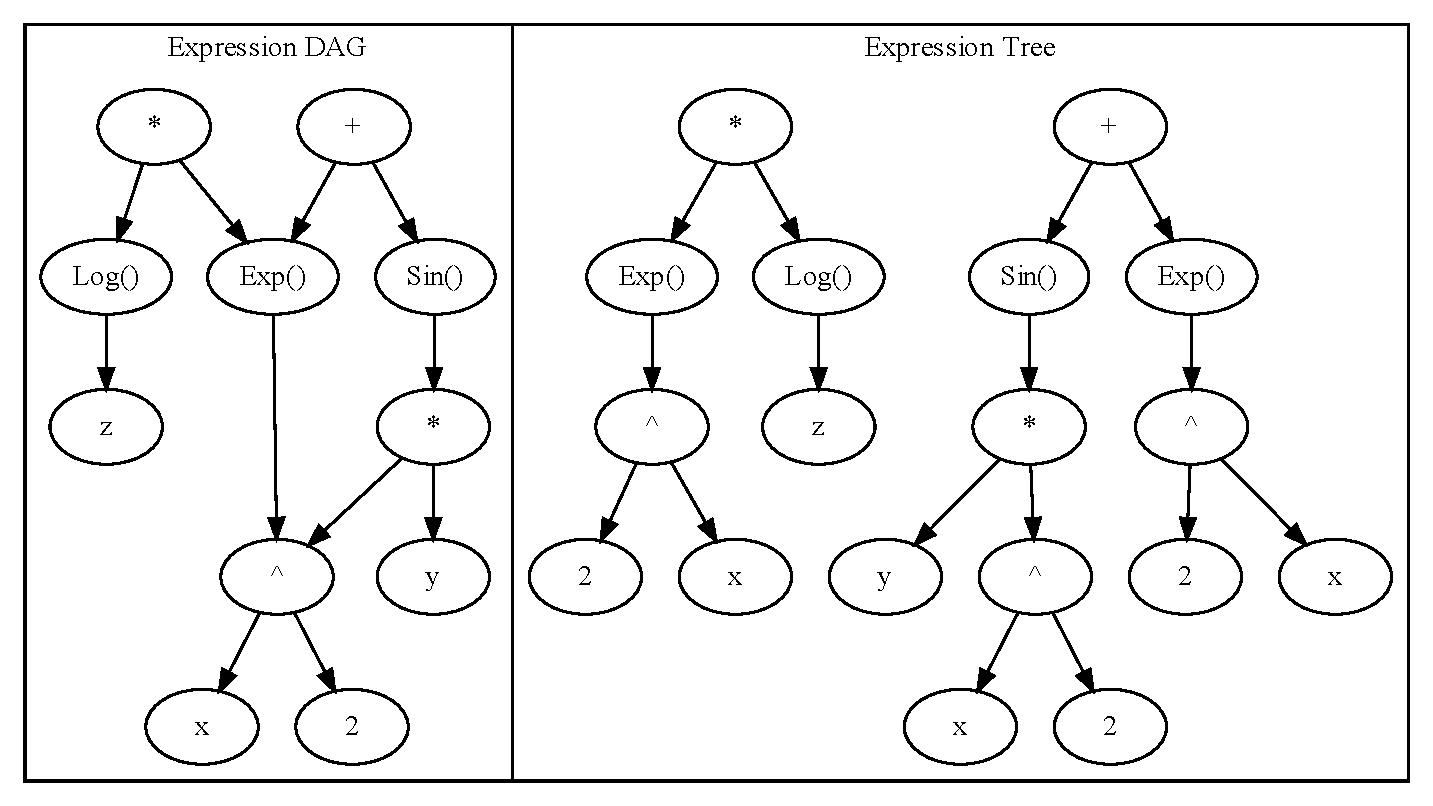
\includegraphics[width=16cm]{images/Clustergraph.gv.pdf}
    \caption{A DAG and Expression Tree representation of Equation \ref{example1}}
    \label{fig:DAGgraph2}
\end{figure}

Below is an example for $F: \mathbb{R}^3 \rightarrow \mathbb{R}^2$ defined by
\begin{equation} \label{example1}
    F \begin{pmatrix}
        x \\ y \\ z
    \end{pmatrix} = \begin{pmatrix}
        \sin (x^2 y) + e^{x^2} \\ e^{x^2} \log z
    \end{pmatrix}
\end{equation}

As in \cite{PoPBook}, we can represent an arithmetic expression as an expression tree. Here we represent each operator, symbol and number in an given expression as nodes in a graph, we denote these as elements. The operands of each element are the children of the node. Notation wise we will represent links out of a node indicating the children of the node, even though expression wise the children are "inputs" to such parent. We can also write an expression as a directed acylic graph which allows us to represent expressions with more than one operators to avoid recursion. An example of the difference between the two can be see in Figure \ref{fig:DAGgraph2}. We from now on will use DAG's to represent expressions as this is essential in lowering runtime and allowing fast computation of complicated expressions. We will presume that ordering of each child is important.

\section{Fundamentals of Algorithmic Differentiation}

Using notation from  \cite{evald}, let $F: \mathbb{R}^n \rightarrow \mathbb{R}^m$ and $F(x) = y$ as in Section 2. Assume $F$ is the composition of a sequence of continuously differentiable elemental functions $(\varphi_i)_{i=1,\ldots, l}$, the derivatives of which can be easily calculated. Hence, $F$ can be represented as a DAG. In our case we will use the elemental functions provided below.

\begin{table}[h]
    \centering
    \begin{tabular}{|c|c|}
        \hline
        Function & Derivative \\
        \hline
        $\sin(u)$ & $\cos(u)$ \\
        $\cos(u)$ & $-\sin(u)$ \\
        $\exp(u) $ & $\exp(u)$ \\
        $\log(u)$ & $1/u$ \\
        $u^k$ & $k u^{k-1}$ \\
        $f(u)g(u)$ & $f'(u)g(u) + f(u)g'(u)$ \\
        $f(u) + g(u)$ & $f'(u) + g'(u)$ \\
        \hline
    \end{tabular}
    \caption{Derivatives of Elemental Functions}
    \label{tab:elemental}
\end{table}

The quantities calculated at each node of the graph during the function evaluation are numbered such that
\begin{equation*}
    [ \underbrace{v_{1-n}, \ldots, v_0}_{x} , v_1, \ldots, v_{l-m}, \underbrace{v_{l-m+1}, \ldots, v_l}_{y}]
\end{equation*}
Using $j \prec i$ to show $v_i$ depends directly on $v_j$ and $j \prec i \Longrightarrow j < i$ then it can be written
\begin{equation*}
    v_i = \varphi_i (v_j)_{j \prec i} \text{ for } \varphi_i : \mathbb{R}^{n_i} \longrightarrow \mathbb{R}
\end{equation*}

\subsection{Forward Mode Algorithmic Differentiation}

We will use the interpretation of forward mode AD given in \cite{dhamarticle}. Assume $x$ is equal to the value a time-dependent $x(t)$ takes at $t=0$. Then define the tangent 
\begin{equation*}
    \dot{x} = \frac{\partial x}{\partial t} \Big|_{t=0}
\end{equation*}
As $y = F(x)$ we calculate the tangent $\dot{y}$ as
\begin{equation*}
    \Dot{y} = \frac{\partial}{\partial t} F(x (t)) \Big|_{t=0} 
    = F'(x (t)) \frac{\partial x}{\partial t} \Big|_{t=0}
    = F'(x) \Dot{x}
    \equiv \Dot{F}(x, \Dot{x})
\end{equation*}
Using the additional notation $u_i = (v_j)_{j \prec i}$ and $\Dot{u}_i = (\Dot{v}_j)_{j \prec i}$, the idea can be applied to an elemental function $\varphi_i : \mathbb{R}^{n_i} \longrightarrow \mathbb{R}$, $v_i = \varphi_i (u_i)$ to get the result
\begin{equation}
    \label{tangentequ}
    \Dot{v_i} = \sum_{j \prec i} \left\{ \Dot{v}_j \cdot \frac{\partial}{\partial v_j} \varphi_i (u_i) \right\} 
    \equiv \Dot{\varphi}_i(u_i, \Dot{u}_i)
\end{equation}

This can be summarised as the general evaluation procedure given in \cite{evald} and given in Table \ref{tab:gep}.

\begin{table}[h]
    \centering
    \begin{tabular}{|lcll|}
        \hline
        $v_{i-n}$ & $\equiv$ & $x_i$ & $i = 1, \ldots, n$ \\
        $\Dot{v}_{i-n}$ & $\equiv$ & $\Dot{x}_i$ & $i = 1, \ldots, n$ \\
        \hline
        $v_{i}$ & $\equiv$ & $v_i = \varphi_i (u_i)$ & $i = 1, \ldots, l$ \\
        $\Dot{v}_{i}$ & $\equiv$ & $\sum_{j \prec i} \left\{ \Dot{v}_j \cdot \frac{\partial}{\partial v_j} \varphi_i (u_i) \right\}$ & $i = 1, \ldots, l$ \\
        \hline
        $v_{l-m+i}$ & $\equiv$ & $y_i$ & $i = 1, \ldots, m$ \\
        $\Dot{v}_{l-m+i}$ & $\equiv$ & $\Dot{y}_i$ & $i = 1, \ldots, m$ \\
        \hline
    \end{tabular}
    \caption{General Evaluation Procedure}
    \label{tab:gep}
\end{table}

When represented on a DAG, forward mode AD begins at the inputs and moves through the graph computing $F$ and $\Dot{F}$ together at each node. For this a concise version of Table \ref{tab:gep} is provided in Table \ref{tab:gtp}.

\begin{table}[h]
    \centering
    \begin{tabular}{|lcll|}
        \hline
        $[v_{i-n}, \Dot{v}_{i-n}]$ & $=$ & $[x_{i}, \Dot{x}_{i}]$ & $i = 1, \ldots, n$ \\
        \hline
        $[v_{i}, \Dot{v}_{i}]$ & $=$ & $[\varphi_i (u_i), \Dot{\varphi}_i(u_i, \Dot{u}_i)]$ & $i = 1, \ldots, l$ \\
        \hline
        $[v_{l-m+1}, \Dot{v}_{l-m+1}]$ & $=$ & $[y_{i}, \Dot{y}_{i}]$ & $i = 1, \ldots, m$ \\
        \hline
    \end{tabular}
    \caption{General Tangent Procedure}
    \label{tab:gtp}
\end{table}

\subsection{Reverse Mode Algorithmic Differentiation}

As in \cite{dhamarticle}, consider for the image of $F$ the hyperplane $\{ y \in \mathbb{R}^m | \Bar{y}^\top y = c\}$ for a given vector $\Bar{y} \in \mathbb{R}^m$ and a given value $c \in \mathbb{R}$. The inverse image of this hyperplane is given by the set $\{ x \in \mathbb{R}^n | \Bar{y}^\top F(x) = c\}$. We can apply the implicit function theorem to this set to calculate the normal to this hyperplane at $x$ as
\begin{equation}
    \Bar{x}^\top = \Bar{y}^\top F'(x) \equiv \Bar{F}(x, \Bar{y})
\end{equation}
This calculation is provided $\Bar{x}^\top$ does not vanish.

Using the additional notation $\Bar{u}_i = (\Bar{v}_j)_{j \prec i}$, we calculate the adjoint function for each elemental function $\varphi : \mathbb{R}^{n_i} \longrightarrow \mathbb{R}$ as
\begin{equation}
    \Bar{u}_i += \Bar{v}_i \nabla \varphi_i (u_i)
\end{equation}

In reverse mode, the tree is first traversed beginning at the inputs and finishing at the outputs, storing the value the elemental function takes at each node. Then, the tree is traversed in the other direction storing the value the adjoint function takes at each node. This produces a the adjoint procedure for computing the first derivative from \cite{dhamarticle}, given below.

\begin{table}[h]
    \centering
    \begin{tabular}{|lcll|}
        \hline
        $v_{i}$ & $=$ & $0$ & $i = 1, \ldots, l$ \\
        \hline
        $[v_{i-1}, \Bar{v}_{i-1}]$ & $=$ & $[x_{i}, \Bar{x}_{i}]$ & $i = 1, \ldots, n$ \\
        \hline
        push$(v_i)$ & & & \\
        $v_{i}$ & $=$ & $v_i = \varphi_i (u_i)$ & $i = 1, \ldots, l$ \\
        \hline
        $v_{l-i}$ & $=$ & $y_{m-1}$ & $i = 1, \ldots, m-1$ \\
        $\Bar{v}_{l-i}$ & $=$ & $\bar{y}_{m-1}$ & $i = 1, \ldots, m-1$ \\
        \hline
        $v_i \leftarrow$ pop$()$ & & & \\
        $\Bar{u}_i$ & $+=$ & $\Bar{v}_i \nabla \varphi_i (u_i)$ & $i = l, \ldots, 1$ \\
        $v_i$ & $=$ & $0$ & \\
        \hline
        $\Bar{v}_{i-n}$ & $=$ & $\Bar{x}_i$ & $i = 1, \ldots, n$ \\
        \hline
    \end{tabular}
    \caption{Adjoint Procedure}
    \label{tab:ap}
\end{table}

\section{Applying Algorithmic Differentiation on DAG's}

If we consider an expression represented by a DAG, then it is very easy to apply the concept of Forward and Reverse mode algorithmic differentiation. Here we can represent each Element/Node denoted $v_i$ as our elementary function $v_i = \varphi_i (v_j)_{j \prec i}$ where now we can view $j \prec i$ to mean that $v_i$ is an operand of $v_j$. Then we can compute our tangents in Equation \ref{tangentequ} by traversing this graph with post-order traversal, calculating both the values, $v_i$, and the tangent values, $\Dot{v_i}$ with respect to a single input variable as we go along

\subsection{Example of Forward Mode Algorithmic Differentiation on a DAG}
Consider an equation

\begin{equation}
    \label{example2}
    f(x,y) = Sin(yx^2) + e^{x^2}
\end{equation}
Say we want to apply our algorithm to the \ref{example2} represented by the DAG in Figure \ref{fig:DAGgraph} evaluating at $x=200$, $y=3$. Here we label the nodes according to the notation used above as seen in Table \ref{example1}. We then traverse the graph in postorder traversal, computing the value of each node as we go along. The results after this pass are seen in Table \ref{example1FM}. Now we will traverse the tree with preorder traversal. We know that first $\dot{v_6} \equiv 1$ and we have all our values calculated from the previous pass, so we get the adjoints as listed in Table \ref{tab:example1RM}

\begin{algorithm}[h]
\caption{ForwardmodeAD algorithm}\label{forwardAD}
\begin{algorithmic}[1]
\Procedure{ForwardmodeAD}{$expression,conditions$}
\State dict = dict()\Comment{}
\For{ each $symbol$ in conditions}
\State Traverse through $expression$, visiting $element$ after its $operands$
    \For{ each node i in expression}
    \State Calculate $v_i$ and $\Dot{v_i}$.t. its $\varphi_i(v_j)_{j \prec i}$ \verb|operands| and \verb|symbol|
    \State dict[symbol] = \verb|expression.adjoint|\Comment{Store the adjoint w.r.t the symbol}
    \EndFor
\EndFor
\State \textbf{return} a dictionary of symbols and their respective \verb|adjoints|
\EndProcedure
\end{algorithmic}
\end{algorithm}


\begin{figure}[h!]
    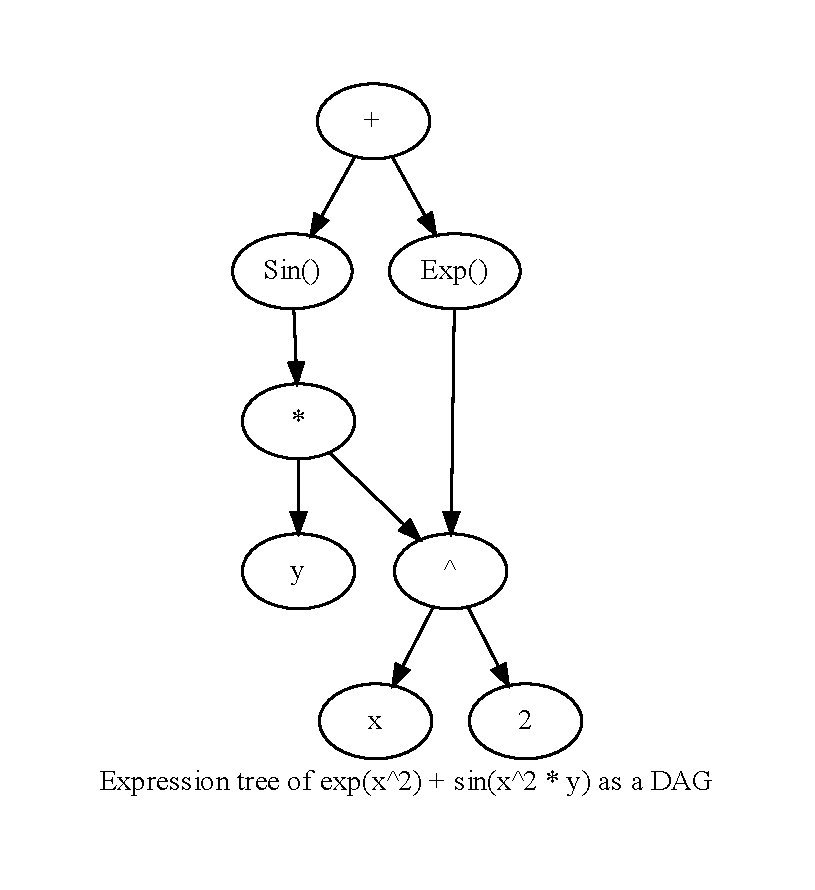
\includegraphics[width=8cm]{images/DAGgraph.gv.pdf}
    \caption{A Tree, left, and DAG, right, representation of expression $Sin(x^2y) + e^{x^2}$. The DAG allows us to avoid unnecessary recursion in the $x^2$ term}
    \label{fig:DAGgraph}
\end{figure}

\begin{table}[h!]
    \centering
    \begin{tabular}{|lcl|lclll|}
        \hline
        $v_{-1}$ & $\equiv$ & $x$ & $\Bar{v}_{-1}$ & $\equiv$ & $\Bar{v_2}\frac{\partial{v_2}}{\partial{v_{-1}}}$ & $=$ & $\Bar{v_2}v_1 {v_{-1}}^{(v_{1}-1)}$\\
        $v_{0}$ & $\equiv$ & $y$ & $\Bar{v}_{0}$ & $\equiv$ & $\Bar{v_3}\frac{\partial{v_3}}{\partial{v_0}}$ & $=$ & $\Bar{v_3}v_2$\\
        \hline
        $v_{1}$ & $\equiv$ & $2$ & $\Bar{v}_{1}$ & $\equiv$ & $\Bar{v_2}\frac{\partial{v_2}}{\partial{v_1}}$ & $=$ & $\Bar{v}_{2}{v_{-1}}^{v_{1}}ln(v_{-1})$\\
        $v_{2}$ & $\equiv$ & ${v_{-1}}^{v_{1}}$ & $\Bar{v}_{2}$ & $\equiv$ & $\Bar{v_3}\frac{\partial{v_3}}{\partial{v_2}} + \Bar{v_5}\frac{\partial{v_5}}{\partial{v_2}}$ & $=$ & $\Bar{v}_{3}v_0 + \Bar{v_5}e^{v_2}$\\
        $v_{3}$ & $\equiv$ & ${v_{0}}*{v_{2}}$ & $\Bar{v}_{3}$ & $\equiv$ & $\Bar{v_4}\frac{\partial{v_4}}{\partial{v_3}}$ & $=$ & $\Bar{v_4}cos(v_2)$\\
        $v_{4}$ & $\equiv$ & $sin(v_3)$ & $\Bar{v}_{4}$ & $\equiv$ & $\Bar{v_6}\frac{\partial{v_6}}{\partial{v_4}}$ & $=$ & $\Bar{v_6}$\\
        $v_{5}$ & $\equiv$ & $e^{v_2}$ & $\Bar{v}_{5}$ & $\equiv$ & $\Bar{v_6}\frac{\partial{v_6}}{\partial{v_5}}$ & $=$ & $\Bar{v_6}$\\
        \hline
        $v_{6}$ & $\equiv$ & $v_5 + v_4$ & $\Bar{v}_{6}$ & $\equiv$ & $\frac{\partial{v_6}}{\partial{v_6}}$ & $=$ & $1$\\
        \hline
    \end{tabular}
    \caption{Table of nodes in Figure \ref{fig:DAGgraph} of Equation \ref{example2}}
    \label{tab:example1}
\end{table}

\begin{table}[h!]
    \centering
    \begin{tabular}{|lclll|}
        \hline
        $v_{-1}$ & $\equiv$ & $x$ & $\equiv$ & 2\\
        $v_{0}$ & $\equiv$ & $y$ & $\equiv$ & 2\\
        \hline
        $v_{1}$ & $\equiv$ & $2$ & $\equiv$ & 2\\
        $v_{2}$ & $\equiv$ & ${v_{-1}}^{v_{1}}$ & $=$ & $ 2^2 = 4$\\
        $v_{3}$ & $\equiv$ & $v_0 * v_2$ & $=$ & $ 2 * 4 = 8$\\
        $v_{4}$ & $\equiv$ & $sin(v_3)$ & $=$ & $ sin(8) \approx 0.989358247$\\
        $v_{5}$ & $\equiv$ & $e^{v_2}$ & $=$ & $ e^4 \approx 54.5982$\\
        \hline
        $v_{6}$ & $\equiv$ & $v_5 + v_4$ & $=$ & $e^4 + sin(8) \approx 55.5875$\\
        \hline
    \end{tabular}
    \caption{Values of Figure \ref{fig:DAGgraph}}
    \label{tab:example1FM}
\end{table}

\begin{table}[h!]
    \centering
    \begin{tabular}{|lclllll|}
        \hline
        $\Bar{v}_{-1}$ & $=$ & $\Bar{v_2}v_1 {v_{-1}}^{(v_{1}-1)}$ & $=$ & $(2cos(8)+e^4) \cdot 2 \cdot 2^{2-1} = 8cos(8)+4e^4$ & $\approx$ & $217.2286$\\
        $\Bar{v}_{0}$ & $=$ & $\Bar{v_3}v_2$ & $=$ & $cos(8)\cdot4 = 4cos(8)$ & $\approx$ & $-0.5820$\\
        \hline
        $\Bar{v}_{1}$ & $=$ & $\Bar{v}_{2}{v_{-1}}^{v_{1}}ln(v_{-1})$ & $=$ & $(2cos(8)+e^4) \cdot 2^2 \cdot ln(2) = 8cos(8)ln(2) +4e^4ln(2)$ & $\approx$ & $63.1932$\\
        $\Bar{v}_{2}$ & $=$ & $\Bar{v}_{3}v_0 + \Bar{v_5}e^{v_2}$ & $=$ & $cos(8) \cdot 2 + 1 \cdot e^{4} = 2cos(8)+e^4$ & $\approx$ & $54.3071$\\
        $\Bar{v}_{3}$ & $=$ & $\Bar{v_4}cos(v_3)$ & $=$ & $1 \cdot cos(8) = cos(8)$ & $\approx$ & $-0.1455$\\
        $\Bar{v}_{4}$ & $=$ & $\Bar{v_6}$ & $=$ & $1$ & $=$ & $1$\\
        $\Bar{v}_{5}$ & $=$ & $\Bar{v_6}$ & $=$ & $1$ & $=$ & $1$\\
        \hline
        $\Bar{v}_{6}$ & $=$ & $1$ & $=$ & $1$ & $=$ & $1$\\
        \hline
    \end{tabular}
    \caption{Adjoints of Figure \ref{fig:DAGgraph}}
    \label{tab:example1RM}
\end{table}

\subsection{Example of Reverse Mode Algorithmic Differentiation on a DAG}



Reverse mode AD consists of a forward pass over the expression tree followed by a reverse pass. The forward pass starts by substituting values into the independent variable(s) and then using these to evaluate the expressions of their parent node(s). This process propagates up the tree to the dependent variable(s). At each node, the evaluation is stored to be used in the reverse pass.

During the reverse pass, the adjoint values of each node, $\bar{w_i} = \frac{\partial{y}}{\partial{w_i}}$, are calculated using the expression:

\begin{equation}
\Bar{v_i} = \sum_{j\in\{\mbox{parent of i}\}} \Bar{v_j}\frac{\partial{v_j}}{\partial{v_i}}
\end{equation}

In the following example, we find the derivative of the function $J = xsin(x+y)$ with respect to the variables $x$ and $y$ when $(x, y) = (1, 1)$.

First, the nodes in the expression tree are labelled in the following way:
\begin{equation}
w_1 = x
\end{equation}
\begin{equation}
w_2 = y
\end{equation}
\begin{equation}
w_3 = w_1 + w_2
\end{equation}
\begin{equation}
w_4 = sin(w_3)
\end{equation}
\begin{equation}
w_5 = w_1 \cdot w_4
\end{equation}
\\\\

Suppose we want to compute $\frac{\partial{J}}{\partial{u}}$ with $u = (x, y) = (1, 1)$, performing the forward pass we obtain $w_1 = 1, w_2 = 1, w_3 = 2, w_4 = sin(2), w_5 = sin(2)$.

For the reverse pass, we seed the value of $\bar{w_5}$ as 1 then, using the formula for $\bar{w_i}$, we obtain:
\begin{equation}
\bar{w_4} = \bar{w_5}\frac{\partial{w_5}}{\partial{w_4}} = \bar{w_5}\cdot w_1 = 1
\end{equation}
\begin{equation}
\bar{w_3} = \bar{w_4}\frac{\partial{w_4}}{\partial{w_3}} = \bar{w_4}\cdot cos(w_3) = cos(2)
\end{equation}
\begin{equation}
\bar{w_2} = \bar{w_3}\frac{\partial{w_3}}{\partial{w_2}} = \bar{w_3}\cdot w_1 = cos(2)
\end{equation}
\begin{equation}
\bar{w_1} = \bar{w_5}\frac{\partial{w_5}}{\partial{w_1}} + \bar{w_3}\frac{\partial{w_3}}{\partial{w_1}} = \bar{w_5}\cdot w_4 + \bar{w_3} = sin(2) + cos(2)
\end{equation}
Therefore, we have computed $\frac{\partial{J}}{\partial{x}}\vert_{(1, 1)} = sin(2) + cos(2)$ and $\frac{\partial{J}}{\partial{y}}\vert_{(1, 1)} = cos(2)$.

\section{Implementation of 1D reverse mode AD in Python}



We first had to define an expressions class that would take the form of a function say:
\begin{equation}
xsin(x+y)
\end{equation}
The expression was then broken down into the elementary functions ($+, -, *, /, sin, cos, exp, log$), from there we define a Directed Acyclic Graph using the earlier elementary functions and parent nodes and the one that follows child nodes, using network x to represent this we can represent (18) by the graph:

\begin{center}
    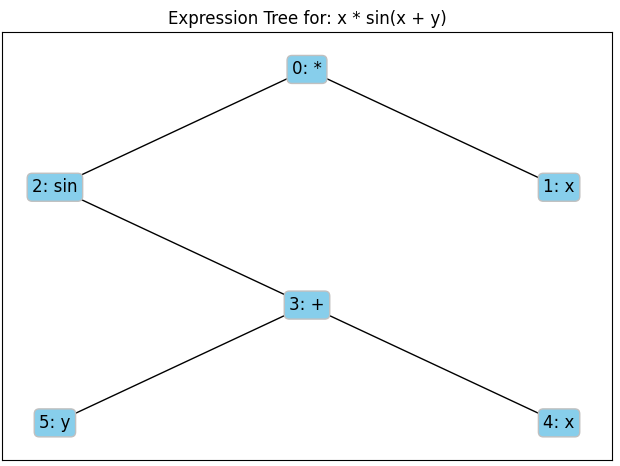
\includegraphics[width=12cm]{images/DAG_1.png}
\end{center}

Now we have the graph, we can operate a forward pass and at each node, we save the value outputted. Taking the example $x = 1$ and $y = 1$ we assign values to nodes as so:

\begin{equation*}
    5: (1, ) 
\end{equation*}
\begin{equation*}
    4: (1, )
\end{equation*}
\begin{equation*}
    3: (2, )
\end{equation*}
\begin{equation*}
    2: (0.90929, )
\end{equation*}
\begin{equation*}
    1: (1, )
\end{equation*}
\begin{equation*}
    0: (0.90929, )
\end{equation*}

Here we are numbering the nodes as they have been in the graph. Having computed these in the first pass we then, using equations (14) - (18) stated above we now calculate the adjoint values by doing a backward pass and assigning them to each node as so:

\begin{equation*}
    5: (1, -0.41615)
\end{equation*}
\begin{equation*}
    4: (1, 0.49315)
\end{equation*}
\begin{equation*}
    3: (2, -0.41615)
\end{equation*}
\begin{equation*}
    2: (0.90929, 1)
\end{equation*}
\begin{equation*}
    1: (1, 0.90929)
\end{equation*}
\begin{equation*}
    0: (0.90929, 1)
\end{equation*}

Returning these values we see that our $\frac{dJ}{dx} = 0.49315 = cos(2) + sin(2)$ is the adjoint value of the x node (node 4) and our $\frac{dJ}{dy} = -0.41615 = cos(2)$ is the adjoint value of the y node (node 5).

We can check the accuracy of our results using 2 methods, first, by using Taylor series we have the equation:
\begin{equation}
    F(x + \epsilon) = F(x) + \frac{dF}{dx} * \epsilon + O(\epsilon ^ 2)
\end{equation}
When we send $\epsilon$ to 0 the term $O(\epsilon)$ goes to 0 meaning we can approximate $\frac{dF}{dx}$ by:

\begin{equation}
    \frac{F(x + \epsilon) - F(x)}{\epsilon}
\end{equation}

We can then subtract this result from our own and the difference should approach 0 as our Epsilon approaches 0. This result is proven by the following graph showing our Taylor error as our Epsilon value approaches 0.

\begin{center}
    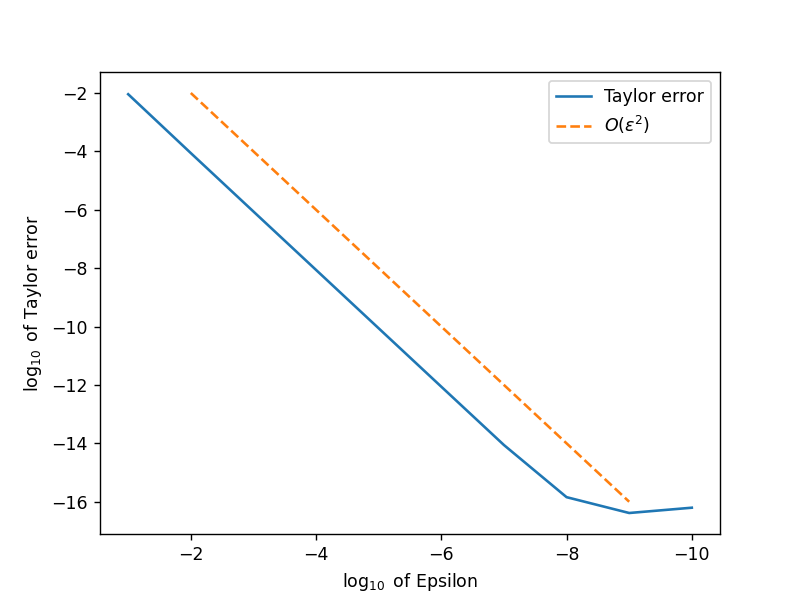
\includegraphics[width=12cm]{images/Taylor_error_1.png}
\end{center}

We can see from this graph that in general as our Epsilon gets smaller so does our Taylor error, as predicted, and our Taylor error plateaus around $10^{-16}$ and this is because machine Epsilon lies in this region.

The other way we check the accuracy is by using the finite difference method, for this we use similar method with a key difference, the formula we will use to approximate the derivative is:

\begin{equation}
    \frac{F(x + \epsilon) + F(x - \epsilon)}{2 \epsilon}
\end{equation}

Using this equation we get an error of order $h^2$ instead of an error of order $h$ found in Taylor error, we see this with the following graph where we see the initial convergence is much faster:

\begin{center}
    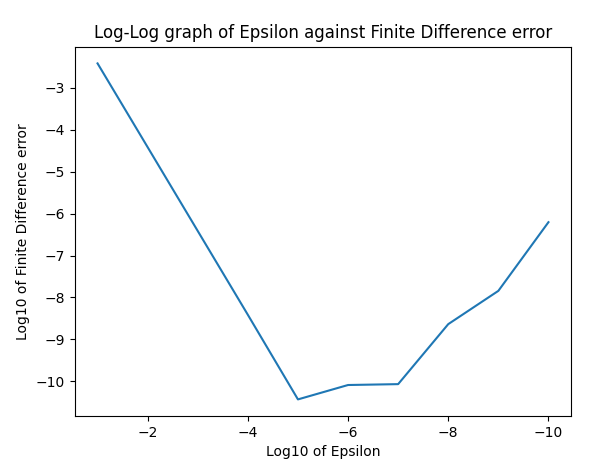
\includegraphics[width=12cm]{images/Finite_Difference_error_1.png}
\end{center}

*** IDK if anybody can explain why it blows up but I can't ***

\section{Extension into numpy arrays}

\section{Applications}

\bibliography{thebibliography}


\section{Dump}

\begin{algorithm}
\caption{Evaluate Postvisitor}\label{evalpostvisitor}
\begin{algorithmic}[1]
\Procedure{Euclid}{$expr,conditions$}\Comment{Expression and conditions}
\State $stack = []$
\State $visited = \{\}$
\State Push $expr$ onto $stack$
\While{$stack$ is not empty}
\State $element \gets stack.pop()$
\For{$operand \in element.opernads$}
\If{$operand \not \in visited$}
\State $unvisited\_children.push(operand)$
\EndIf
\EndFor
\If{$unvisited\_children not empty$}
\State $stack.push(element)$
\State $stack.push(unvisited\_children)$
\Else
\State $visited[element] \gets$ evaluate$(element, *(visited[operand]$ for $operand$ in $element.opernads), symbol\_map = conditions)$
\State $element.storedvalue \gets visited[element]$
\EndIf
\EndWhile\label{euclidendwhile}
\State \textbf{return} $visited[expr]$
\EndProcedure
\end{algorithmic}
\end{algorithm}


Algorithm 2 provides the pseudocode behind the \verb|EvaluatePostvisitor| function. This will traverse through the tree in postorder and evaluate each node as it goes along. The \verb|evaluate| function for a node itself will depend on the \verb|type()| of node (what its operators are), its already evaluated operands, and the initial conditions. For example \verb|Add(x, y)| with initial conditions \verb|x = 2, y = 3| will be evaluated by evaluating \verb|x| and \verb|y| first, which will both \verb|x.storedvalue = 2| and \verb|y.storedvalue = 3|. Then \verb|Add(x, y)| will be evaluated and \verb|Add(x, y).storedvalue() = 5|. Finally, the function will return $5$
\\\\
Using the graph below we can see what our function looks like after our EvaluatePostvisitor function.
\\\\
Next Algorithm 3 provides the pseudocode behind the \verb|AdjointPrevisitor()| function, this will now traverse through the tree in preorder, evaluating the adjoints of the operands of the node as it goes along. This different \verb|evaluate_adjoint| function for a node itself will depend on the \verb|type()| of node (what its operators are), and the \verb|storedvalue| for its operands. Once this function has evaluated the adjoint of an operand, it will recursively call itself again on its operand, this allows us to do preorder traversal on our expression tree.
\\\\
Using the graph below we can see what our function looks like after our AdjointPrevisitor function.
\\\\
Next Algorithm 4 provides the pseudocode behind the \verb|ReversemodeAD()| which takes in \verb|expression| and \verb|conditions| which are the expression and conditions to evaluate the derivative at and returns a dictionary of the partial derivatives of \verb|expression| w.r.t. the symbols in \verb|expression|. It does this by simply running our \verb|EvaluatePostvisitor(expression, conditions)|. And then running \verb|AdjointPrevisitor(expression)|. Once both are run we now have adjoints attached to every node/element in expression. It will then return a dictionary of the symbols and their respective adjoints (which are the partial derivatives)

\begin{algorithm}[h]
\caption{EvaluatePostvisitor function}\label{EvaluatePostvisitor}
\begin{algorithmic}[1]
\Procedure{EvaluatePostvisitor}{$expression,conditions$}
\State non recursively traverse through $expression$, visiting $element$ after its $operands$
\For{each $element$ in expression}
\State evaluate the value of $element$ w.r.t. its type, $operands$, and $conditions$
\State set $element$.$storedvalue$ attribute to this value
\EndFor
\State \textbf{return} $expression$.$storedvalue$ attribute 
\EndProcedure
\end{algorithmic}
\end{algorithm}


\begin{algorithm}
\caption{AdjointPrevisitor function}\label{AdjointPrevisitor}
\begin{algorithmic}[1]
\Procedure{AdjointPrevisitor}{$expression$}
\State traverse through \verb|expression|, visiting \verb|element| before its \verb|operands|
\For{each \verb|operand in expression.operands|}
\State evaluate the \verb|adjoint| of \verb|operand| w.r.t. \verb|expression|'s type and its \verb|operands|
\State update and add this value to \verb|operand.adjoint|\Comment{Add value to allow recursion}
\State run \verb|AdjointPrevisitor(operand)|
\EndFor
\EndProcedure
\end{algorithmic}
\end{algorithm}

\begin{algorithm}
\caption{ReversemodeAD algorithm}\label{reverseAD}
\begin{algorithmic}[1]
\Procedure{ReversemodeAD}{$expression,conditions$}
\State run \verb|EvaluatePostvisitor(expression, conditions)|
\State run \verb|AdjointPrevisitor(expression)|
\State \textbf{return} a dictionary of Symbols and their respective \verb|adjoints|
\EndProcedure
\end{algorithmic}
\end{algorithm}

\begin{center}
    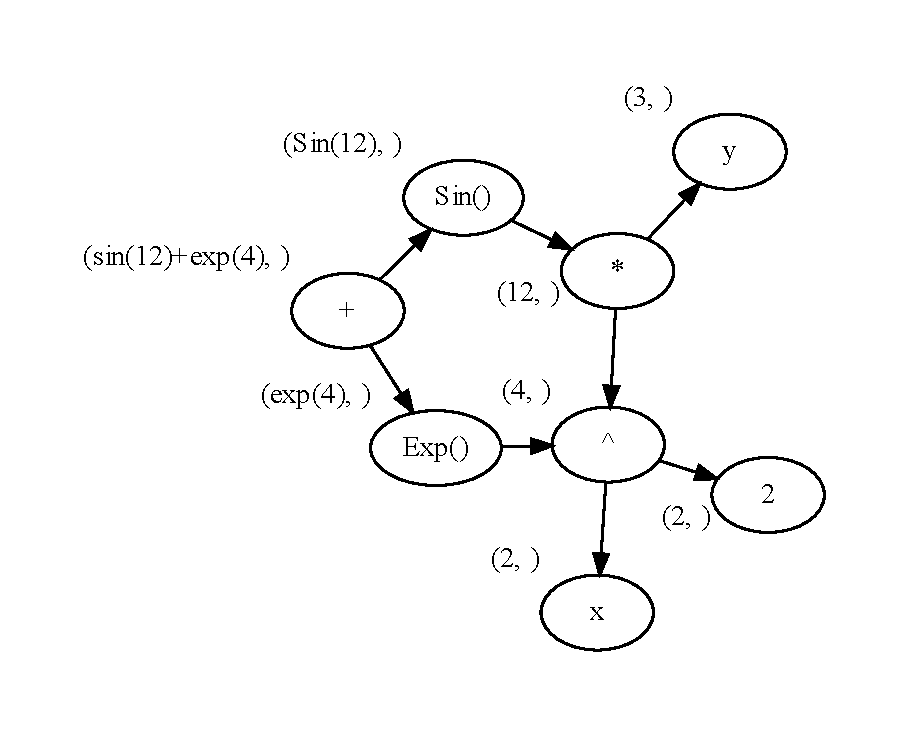
\includegraphics[width=12cm]{images/graph.gv.pdf}
\end{center}

\begin{algorithm}
\caption{ForwardmodeAD algorithm}\label{forwardAD}
\begin{algorithmic}[1]
\Procedure{ForwardmodeAD}{$expression,conditions$}
\State dict = dict()
\For{ each symbol in conditions}
\State non recursively traverse through $expression$, visiting $element$ after its $operands$
    \For{ each \verb|element| in expression}
    \State set \verb|element.adjoint = 0|\Comment{So we don't use adjoints calculated for other symbols}
    \State evaluate value and \verb|adjoint| of \verb|element| w.r.t. its \verb|type()|, \verb|operands| and \verb|symbol|
    \State dict[symbol] = \verb|expression.adjoint|\Comment{Store the adjoint w.r.t the symbol}
    \EndFor
\EndFor
\State \textbf{return} a dictionary of symbols and their respective \verb|adjoints|
\EndProcedure
\end{algorithmic}
\end{algorithm}



\section{Max Dump}

If $n=m=1$ then
\begin{equation*}
    f'(x) \approx \frac{f(x+h)-f(x)}{h}
\end{equation*}
and from \cite{quarteroni} it is known that
\begin{equation*}
    f'(x) - \frac{f(x+h)-f(x)}{h} = - \frac{h}{2} f''(\xi)
\end{equation*}
where $\xi \in (x, x+h)$.

\textbf{REFERENCE: https://rufflewind.com/2016-12-30/reverse-mode-automatic-differentiation}


\end{document}